\documentclass[tikz]{standalone}
    \usepackage{tikz}
    \usetikzlibrary{positioning, graphs}
    \usetikzlibrary{graphs.standard}
    \begin{document}
    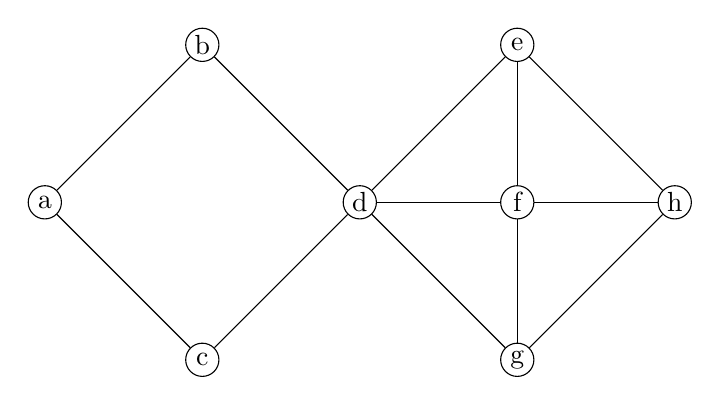
\begin{tikzpicture}
    \begin{scope}
            [vertex/.style={draw,circle,inner sep = 0em, minimum size = 1.2em},
             edgelabel/.style = {fill = white, inner sep = 0.1em, font=\small}]
            \node[vertex] (a) at (0,0) {a};
            \node[vertex] (b) at (2,2) {b};
            \node[vertex] (c) at (2,-2) {c};
            \node[vertex] (d) at (4,0) {d};
            \node[vertex] (e) at (6,2) {e};
            \node[vertex] (f) at (6,0) {f};
            \node[vertex] (g) at (6,-2) {g};
            \node[vertex] (h) at (8,0) {h};
            
            \draw[-] (a) to (b);
            \draw[-] (a) to (c);
            \draw[-] (b) to (d);
            \draw[-] (c) to (d);
            \draw[-] (d) to (e);
            \draw[-] (d) to (f);
            \draw[-] (d) to (g);
            \draw[-] (e) to (h);
            \draw[-] (e) to (f);
            \draw[-] (f) to (g);
            \draw[-] (f) to (h);
            \draw[-] (g) to (h);
    \end{scope}
    \end{tikzpicture}
    \end{document}